\documentclass[12pt,a4paper]{memoir}
% \documentclass[titlepage,12pt,a4paper]{book}

% substituir linha seguinte por 
% \usepackage[english]{babel} 
% se o relatório for escrito na língua inglesa.
\usepackage[portuguese]{babel}

\usepackage{amssymb}


% \usepackage[utf8]{inputenc}
\usepackage[T1]{fontenc}

\usepackage{makeidx}
\usepackage{xspace}
\usepackage{graphicx,color,times}
\usepackage{fancyhdr}
% \usepackage{pxfonts}
% \usepackage{times}
% \usepackage{mathptm}
% \usepackage{amssymb}
% \usepackage{amsfonts}

\usepackage{amsmath}
\usepackage{latexsym}
\usepackage[printonlyused]{acronym}
\usepackage{float}
\usepackage{listings}
\usepackage{tocbibind}
\usepackage{natbib}
\usepackage{hyperref}

% \usepackage{glossaries}
% \makeglossaries

% \renewcommand{\ttdefault}{phv}

\pagestyle{fancy}
\renewcommand{\chaptermark}[1]{\markboth{#1}{}}
\renewcommand{\sectionmark}[1]{\markright{\thesection\ #1}}
\fancyhf{} \fancyhead[LE,RO]{\bfseries\thepage}
\fancyhead[LO]{\bfseries\rightmark}
\fancyhead[RE]{\bfseries\leftmark}
\renewcommand{\headrulewidth}{0.5pt}
\renewcommand{\footrulewidth}{0pt}
\setlength{\headheight}{15.6pt}
\setlength{\marginparsep}{0cm}
\setlength{\marginparwidth}{0cm}
\setlength{\marginparpush}{0cm}
\addtolength{\hoffset}{-1.0cm}
\addtolength{\oddsidemargin}{\evensidemargin}
\addtolength{\oddsidemargin}{0.5cm}
\addtolength{\evensidemargin}{-0.5cm}


\usepackage{fix-cm}
\usepackage{fourier}
\usepackage[scaled=.92]{helvet}
\definecolor{ChapGrey}{rgb}{0.6,0.6,0.6}
\newcommand{\LargeFont}{
  \usefont{\encodingdefault}{\rmdefault}{b}{n}
  \fontsize{60}{80}\selectfont\color{ChapGrey}
  }
\makeatletter
\makechapterstyle{GreyNum}{
  \renewcommand{\chapnamefont}{\large\sffamily\bfseries\itshape}
  \renewcommand{\chapnumfont}{\LargeFont}
  \renewcommand{\chaptitlefont}{\Huge\sffamily\bfseries\itshape}
  \setlength{\beforechapskip}{0pt}
  \setlength{\midchapskip}{40pt}
  \setlength{\afterchapskip}{60pt}
  \renewcommand\chapterheadstart{\vspace*{\beforechapskip}}
  \renewcommand\printchaptername{
  \begin{tabular}{@{}c@{}}
    \chapnamefont \@chapapp\\}
    \renewcommand\chapternamenum{\noalign{\vskip 2ex}}
    \renewcommand\printchapternum{\chapnumfont\thechapter\par}
    \renewcommand\afterchapternum{
  \end{tabular}
  \par\nobreak\vskip\midchapskip}
  \renewcommand\printchapternonum{}
  \renewcommand\printchaptertitle[1]{
  {\chaptitlefont{##1}\par}}
  \renewcommand\afterchaptertitle{\par\nobreak\vskip \afterchapskip}
}
\makeatother
\chapterstyle{GreyNum}

\setcounter{tocdepth}{3}
\setsecnumdepth{subsubsection}

\renewcommand{\ttdefault}{lmtt}


% NEW COLORS
\definecolor{dark}{gray}{0.25}
\definecolor{lgray}{gray}{0.9}
\definecolor{dkblue}{rgb}{0,0.13,0.4}
\definecolor{dkgreen}{rgb}{0,0.6,0}
\definecolor{gray}{rgb}{0.5,0.5,0.5}
\definecolor{mauve}{rgb}{0.58,0,0.82}

\lstset{ %
  language=C,                    basicstyle=\footnotesize,
  numbers=none,                  numberstyle=\tiny\color{gray}, 
  stepnumber=1,                  numbersep=5pt,
  backgroundcolor=\color{white}, showspaces=false,
  showstringspaces=false,        showtabs=false,
  frame=single,                  rulecolor=\color{black},
  tabsize=2,                     captionpos=b,
  breaklines=true,               breakatwhitespace=false,
  title=\lstname,                keywordstyle=\color{blue},
  commentstyle=\color{dkgreen},  stringstyle=\color{mauve},
  escapeinside={\%*}{*)},        morekeywords={*},
  belowskip=0cm
}

\renewcommand{\lstlistingname}{Excerto de Código}
\renewcommand{\lstlistlistingname}{Lista de Excertos de Código}

\renewcommand{\today}{\day \ifcase \month \or Janeiro\or Fevereiro\or Março\or %
Abril\or Maio\or Junho\or Julho\or Agosto\or Setembro\or Outubro\or Novembro\or %
Dezembro\fi de \number \year} 



\begin{document}

\thispagestyle{empty}
\setcounter{page}{-1}

\begin{center}
\begin{Huge}
\textbf{Universidade da Beira Interior}
\end{Huge}
\end{center}

\begin{center}
\begin{Huge}
Departamento de Informática
\end{Huge}
\end{center}

\vspace{0,07cm}
\begin{figure}[!htb]
\centering

\includegraphics[width=191pt]{ubi-fe-di.png}
\end{figure}

\vspace{0.5cm}
\begin{center}
\begin{Large}
\textbf{N\textordmasculine{} 2 - 2020: \emph{  $\alpha$steroids - Alpha Defense Team}}
\end{Large}
\end{center}


\vspace{0.5cm}
\begin{center}
\begin{normalsize}
\begin{large}
Elaborado por:
\end{large}
\end{normalsize}
\end{center}

\vspace{0.2cm}
\begin{center}
\begin{large}
\textbf{Rúben Guilherme, nº 41059}
\linebreak
\textbf{Paulo Duarte, nº 41853}
\end{large}
\end{center}

\vspace{0,5cm}
\begin{center}
\begin{normalsize}
\begin{large}
Orientador:
\end{large}
\end{normalsize}
\end{center}

\vspace{0.2cm}
\begin{center}
\begin{large}
\textbf{Professor/a Doutor/a Abel Gomes}
\end{large}
\end{center}



\vspace{0.5cm}
\begin{center}
\begin{normalsize}
\today
\end{normalsize}
\end{center}



\tableofcontents

\clearpage{\thispagestyle{empty}\clearpage

% #   ATENÇÃO
% Se existirem trechos de código, descomentar as seguintes linhas
% \clearpage{\thispagestyle{empty}\cleardoublepage}
% \lstlistoflistings

% \clearpage{\pagestyle{empty}\cleardoublepage}
% \chapter*{Glossário}
\makeglossaries

\newglossaryentry{.NET Framework}
{
  name={.NET Framework},
  description={É uma plataforma para desenvolvimento e funcionamento de aplicações desenvolvida pela Microsoft.}
}

\newglossaryentry{ASP.NET}
{
  name={ASP .Net},
  description={É uma plataforma da Microsoft para o desenvolvimento de aplicações Web e é o sucessor da tecnologia ASP.}
}

\newglossaryentry{CS}
{
  name={C\#},
  description={Lê-se \textit{C Sharp} e é uma linguagem de programação orientada a objectos, desenvolvida pela Microsoft, inicialmente para a plataforma .NET. O C\# é inspirado na junção entre as linguagens C++ e Java.}
}


\newglossaryentry{Java}
{
  name={JAVA},
  description={É uma linguagem de programação orientada a objectos, desenvolvida pela Sun Microsystems na década de 90. Hoje pertence à empresa Oracle.}
}


\newglossaryentry{OpenDMTP}
{
  name={OpenDMTP},
  description={\textit{Open Device Monitoring and Tracking Protocol} é um protocolo e uma \textit{framework} abertos que permite a comunicação bidireccional entre servidores e clientes através da internet.}
}


\newglossaryentry{OpenGTS}
{
  name={Open GTS},
  description={É o primeiro projecto \textit{Open Source} \textit{Web-Based} para controlo de frotas por GPS.}
}


\newglossaryentry{VS2010}
{
  name={Visual Studio 2010},
  description={\textit{Microsoft Visual Studio 2010} é um sistema de desenvolvimento desenvolvido pela Microsoft e é dedicado ao Framework .NET, que contem um conjunto de ferramentas de desenvolvimento projectadas para auxiliar os programadores a enfrentarem desafios complexos.}
}


\newglossaryentry{WebS}
{
	name={Web Service},
	description={Web services são aplicações modulares auto-descritas e auto-contidas, que permitem a integração de sistemas e a comunicação entre aplicações de diferentes tipos.}
}


\newglossaryentry{WebBased}
{
	name={Web Based},
	description={Aplicação desenvolvida para a Web.}
}

\newglossaryentry{Roaming}
{
	name={Roaming},
	description={Define a possibilidade de um utilizador de uma determinada rede obter rede/conecção fora da área geográfica onde foi registado.}
}


\newglossaryentry{Smartphone}
{
	name={Smartphone},
	description={Smartphone é um telefone móvel que contem muitas das principais tecnologias de comunicação e serviços que existem nos computadores pessoais, como acesso a e-mails, serviços de mensagens instantâneas, internet, GPS, entre outros.}
}

\newglossaryentry{TCPIP}
{
	name={TCP/IP},
	description={É um conjunto de protocolos de comunicação entre computadores ligados rede. O nome TCP/IP surge da união entre dois protocolos: o TCP (Transmission Control Protocol) e o protocolo IP (Internet Protocol).}
}

\newglossaryentry{Firewall}
{
	name={Firewall},
	description={É o nome criado para definir um dispositivo para uma rede de computadores que tem como objectivo criar uma política de segurança num determinado ponto de controlo da rede.}
}

\newglossaryentry{JavaScript}
{
	name={JavaScript},
	description={É uma linguagem de programação baseada na linguagem de programação ECMAScript. Actualmente é a linguagem de programação mais utilizada em \textit{``Client-Side''} nos \textit{browsers}.}
}

\newglossaryentry{Flash}
{
	name={Flash},
	description={Desenvolvido pela Macromedia, o Flash é um software utilizado para criação de animações interactivas que funcionam incorporadas em \textit{Browsers}, \textit{Desktop}, \textit{Smartphones}, \textit{Tablets}, e Televisores.}
}


\newglossaryentry{StoredProcedure}
{
	name={Stored Procedure },
	description={É o nome dado a um conjunto de comandos numa base de dados de forma a simplificar a sua utilização.}
}

\newglossaryentry{SQLS}
{
	name={SQL Server 2008},
	description={É um sistema de gestão de base de dados relacional criado pela Microsoft.}
}

\newglossaryentry{Firm}
{
	name={Firmware},
	description={É o conjunto de instruções operacionais programadas directamente no \textit{hardware} de um equipamento electrónico.}
}

\newglossaryentry{browser}
{
	name={Browser},
	description={É um programa de computador que possibilita aos utilizadores uma interacção com documentos virtuais da Internet, também conhecidos como páginas Web.}
}



\mainmatter
\acresetall
\chapter{Introdução}
\label{chap:intro}

\section{Motivação}
\label{sec:mot}
Este projeto foi desenvolvido, no âmbito da disciplina de Computação Gráfica lecionada pelo professor Abel Gomes, com o intuito de desenvolver e aperfeiçoar as técnicas aprendidas ao longo do semestre.

\section{História do jogo}
\label{sec:hist}
\begin{enumerate}
\item \textbf{Quem é o jogador?} -- O jogador faz parte da equipa de defesa Alpha da base espacial UPT-2. Esta base está a navegar por uma cintura de asteroides e devido a isso está a ser atacada por naves inimigas. O jogador deve proteger o caminho da base espacial contra os asteroides e eventuais naves inimigas.
\item \textbf{Quem é o inimigo?} -- O inimigo faz parte dos planetas que ambicionam destruir a nossa presença no Universo. Depois da destruição da Terra alguns planetas decidiram revoltar-se contra a União Planetária da Terra, criada para unir e guiar as várias nações terráqueas. Estes não querem mais um inimigo a conquistar o cosmos e estão dispostos a tudo para eliminar os humanos.
\item \textbf{Porquê?} -- Alienígenas estão a atacar o planeta Terra com o intuito de dizimar a raça humana. Assim sendo, os terráqueos não têm outra opção senão fugir, uma vez que a tecnologia dos extraterrestres é muito superior à dos humanos.
\item \textbf{Objetivo?} -- Fugir do planeta Terra atravessando a cintura de asteroides.
\item \textbf{Onde?} -- Sistema Solar - Cintura de asteróides
\end{enumerate}
\clearpage{\thispagestyle{empty}\cleardoublepage}
\chapter{Tecnologias e Ferramentas Utilizadas}
\label{chap:tecno-ferra}

\section{OpenGL}
\label{chap2:sec:opengl}
OpenGL é a API utilizada para o desenvolvimento do jogo Asteroids em 3D.

\section{GLFW}
\label{chap2:sec:glfw}
A biblioteca GLFW é utilizada para que nos seja possível criar e gerir janelas e interagir com o teclado e com o rato. 

\section{GLM}
\label{chap2:sec:glm}
A biblioteca GLM é utilizada para que consigamos extender o nosso conjuntos de funções matemáticas. 

\section{GLAD}
\label{chap2:sec:glad}
O Glad é utilizado para carregar algumas linguagens necessárias para a implementação do programa nomeadamente o GL.

\section{ASSIMP}
\label{chap2:sec:assimp}
A biblioteca ASSIMP é utilizada para importar os nossos objetos 3D.

\section{FreeType}
\label{chap2:sec:freetype}
A biblioteca FreeType é utilizada para que possamos ler fontes de texto e convertê-las de forma a que as possamos utilizar no OpenGL.

\section{Blender}
\label{chap2:sec:blender}
Utilizámos o Blender para modelar e texturizar os nossos objetos.
\clearpage{\thispagestyle{empty}\cleardoublepage}
\chapter{Desenvolvimento e Implementação}
% Os titulos dados aos capítulos são meros exemplos. Cada relatório deve adequar-se ao projeto desenvolvido.
\label{chap:dens-imp}

\section{Gestão do projeto}
\label{chap4:sec:gestao-proj}


\section{Parte Técnica}
\label{chap4:sec:p-tecnica}

\subsection{Modelação}

\subsection{Interação}

\subsection{Iluminação}

\subsection{Texturização}


\section{Funcionalidades Extra}
\label{chap4:sec:func-extra}

\subsection{Menu}

\subsection{Sistemas de Pontuação}
\clearpage{\thispagestyle{empty}\cleardoublepage}
\chapter{Descrição do funcionamento do software}
% Os titulos dados aos capítulos são meros exemplos. Cada relatório deve adequar-se ao projeto desenvolvido.
\label{chap:desc-soft}
O jogo consiste numa nave que, controlada pelo jogador através do rato e do teclado, tem de destruir os asteróides existentes. Caso a nave não consiga destruir ou desviar-se dos asteróides, esta vai perdendo vida até ser destruída.
\linebreak
\linebreak
A nave movimenta-se num mapa esférico com limites bem definidos, caso a nave se movimente para fora dos limites do mapa, inicialmente aparecerá uma mensagem de aviso que se ignorada pelo jogador, este perderá o jogo tendo de começar de novo.
\linebreak
\linebreak
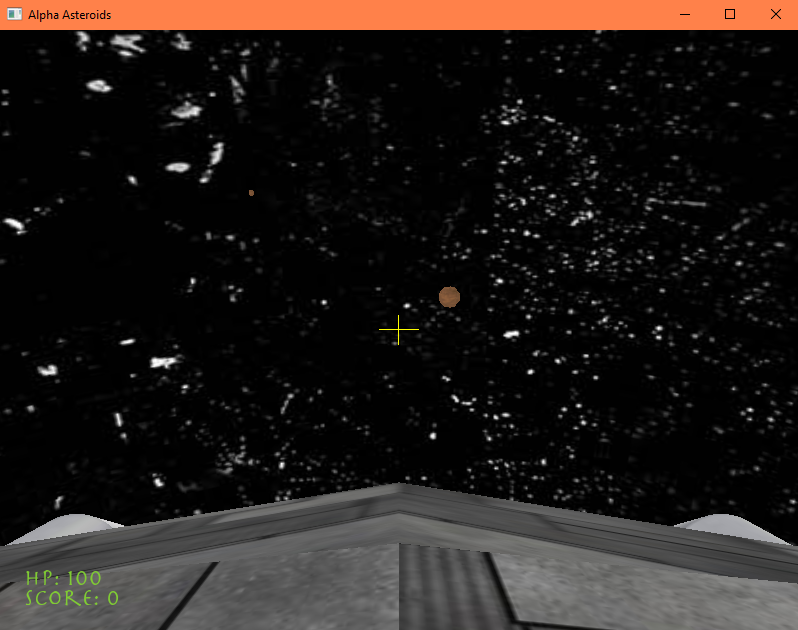
\includegraphics[scale=0.5]{jogo.png}
\clearpage{\thispagestyle{empty}\cleardoublepage}
\chapter{Conclusões e Trabalho Futuro}
\label{chap:conc-trab-futuro}

\section{Conclusões Principais}
\label{sec:conc-princ}

Esta secção contém a resposta à questão: \\
\emph{Quais foram as conclusões princípais a que o(a) aluno(a) chegou no fim deste trabalho?}

\section{Trabalho Futuro}
\label{sec:trab-futuro}

Esta secção responde a questões como:\\
\emph{O que é que ficou por fazer, e porque?}\\
\emph{O que é que seria interessante fazer, mas não foi feito por não ser exatamente o objetivo deste trabalho?}\\
\emph{Em que outros casos ou situações ou cenários -- que não foram estudados no contexto deste projeto por não ser seu objetivo -- é que o trabalho aqui descrito pode ter aplicações interessantes e porque?}
\clearpage{\thispagestyle{empty}\cleardoublepage}
\chapter{Bibliografia}
% Os titulos dados aos capítulos são meros exemplos. Cada relatório deve adequar-se ao projeto desenvolvido.
\label{chap:bibliografia}
1. https://learnopengl.com/In-Practice/2D-Game/Levels
\linebreak
2. https://learnopengl.com/Getting-started/Transformations
\linebreak
3. https://learnopengl.com/Model-Loading/Assimp
\linebreak
4. https://learnopengl.com/Model-Loading/Mesh
\linebreak
5. https://learnopengl.com/Model-Loading/Model
\linebreak
6. https://learnopengl.com/Getting-started/Camera
\linebreak
7. https://github.com/lucatironi/cpp-gl-asteroids
\linebreak
8. https://www.cplusplus.com/reference/vector/vector/
\linebreak
9. https://www.glfw.org/docs/3.3/input_guide.html
\linebreak
10. https://cc0textures.com/categories
\linebreak
11. https://developer.mozilla.org/en-US/docs/Games/Techniques/3D_collision_detection
\linebreak
12. http://www.cplusplus.com/reference/cmath/sqrt/
\clearpage{\thispagestyle{empty}\cleardoublepage}
% SE EXISTIREM APENDICES, DESCOMENTAR O QUE ESTÁ EM BAIXO
% \appendix
% \include{apendice1}
% \clearpage{\pagestyle{empty}\cleardoublepage}
% \include{continuacao}
% \clearpage{\pagestyle{empty}\cleardoublepage}
% \include{apendice2}
% \clearpage{\pagestyle{empty}\cleardoublepage}
% \include{apendice3}
% \clearpage{\pagestyle{empty}\cleardoublepage}

\backmatter

\end{document}